% \begin{document}
\chapter{Reti di Flusso}
Lo sbilanciamento e' un parametro del problema.

Ad ogni arco associamo:
\begin{itemize}
\item Un \textbf{costo}, che indica il costo per unita' di bene per attraversare il canale
\item Una \textbf{capacita' inferiore} $ l_{ij} $ 
\item Una \textbf{capacita' superiore} $ u_{ij} $
\end{itemize}

Le ultime due sono non negative, dato che il flusso su un canale non puo' essere negativo.

\begin{center}
  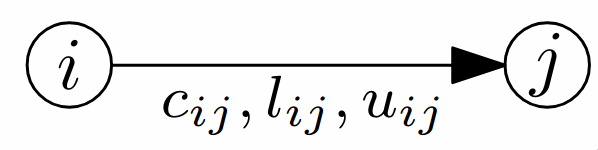
\includegraphics[width=0.5\textwidth]{img/2025-03-05-09-34-49.png}
\end{center}

Il \textbf{flusso} e' proprio la soluzione che vogliamo trovare, ed e' in pratica l'assegnamento di numeri reali a ogni arco, per indicare quanto vogliamo far scorrere per quel tubo.

Il costo complessivo del flusso e' dato da:
\[
  \sum_{(i,j) \in A} c_{ij}x_{ij}
\]

Vincoli:
\begin{itemize}
\item \textit{Domanda e offerta globale si equivalgono}:
  \[
  \sum_{i \in D}b_i = - \sum_{i \in O} b_i
  \]
  Dove $ D = \{b_i \in N | b_i > 0\} $ e $ O = \{b_i \in N | b_i < 0\} $. Per quelli nulli, tanto vale non metterli da nessuna parte per non creare asimmetria inutile.
\item \textit{Il flusso si conserva}:
  \[
 lol 
  \]
dove
\begin{align*}
  BS(i) = \{(k,i) | (k,i) \in A\}\\
  FS(i) = \{(i,k) | (i,k) \in A\}
\end{align*}
Ovvero cio' che entra nel nodo e' uguale a cio' che esce piu' lo sbilanciamento.
\item Il flusso deve essere ammissibile:
  \[
    l_{ij} \leq x_{ij} \leq u_{ij} \quad \forall (i,j) \in A
  \]
\end{itemize}

Perche' mai dovremmo studiare sta roba?
\begin{itemize}
\item \textbf{Espressivita'}: permette di catturare un range di problemi concreti abbastanza grande
\item \textbf{Complessita'}: esistono algoritmi che risolvono questo tipo di problemi con complessita' polinomiale abbastanza basso. A Ugo questo fa molto piacere :)
\end{itemize}

Ipotesi semplificative -> ipotesi che ci permettono di non usare il caso generale, ma che ci semplificano la vita \textbf{senza} perdere espressivita'

Come ad esempio nel caso in cui le capacita' inferiori sono nulle, che e' una situazione a cui possiamo arrivare \textbf{anche da grafi che non hanno questa caratteristica}:

\begin{itemize}
\item Si sottrae $ l_{ij} $ a $ b_j $ e a $ u_{ij} $
\item Si aggiunge $ l_{ij} $ a $ b_i $
\item Occorre aggiungere la quantita'
  \[
    \sum_{(i,j) \in A} c_{ij}l_{ij}
  \]
  che e' il costo della quantita' che necessariamente deve passare. Notare che non cambia la soluzione ottima, ma solo il valore ottimo.
\end{itemize}

Quindi, ad un flusso 

\section{Problema del Flusso di Costo Minimo}

Il costo del flusso e' la funzione obbitettivo da minimizzare e le capacita' inferiori sono nulle. 

\[
0 \leq x \leq u \quad Ex = b
\]

dove

\begin{itemize}
  \item $ E \in \mathbb{R} ^{|N| \times |A|} $ e' una matrice di incidenza fra nodi e archi. Ha solo valori 0, -1 e 1
\end{itemize}

Stiamo solo riscrivendo i vincoli di prima in forma matriciale in modo semplice.

Puo' essere utile assumere che esiste un solo pozzo e una sola sorgente, che vengono poi collegati con archi fittizi (a costo nullo e capacita' pari allo sbilanciamento dei pozzi/sorgenti effettivi!) a quelli effettivi

Perche' non possiamo dire anche che i nodi hanno una capacita'? Perche' di fatto non succede nulla, perche' puo' essere trasformata in una rete equivalente dove i nodi non ce l'hanno:
\begin{itemize}
\item Divido il nodo in due nodi collegati da un arco fittizio
\item Uno dei nodi riceve, l'altro manda
\item Sono collegati da un arco fittizzio dove $ l_{jk} $ e $ u_{jk} $ corrisponono alla capacita' del nodo originale
\end{itemize}

\subsection{Problema di Flusso Massimo}
Vogliamo massimizzare il flusso, non minimizzare il costo.

Vogliamo far arrivare piu' flusso possibile al pozzo, tenendo conto solo ai vincoli sula capacita' superiore

Funzione obbiettivo e vincoli:

Perche' sta roba e' un caso particolare di MCF? Cio' che prima era un parametro diventa una variabile! Facciamo cosi:
\begin{itemize}
\item I costi sono nulli
\item Gli sbilanciamenti sono nulli
\item Si aggiunge un arco da $ t $ a $ s $ 

\subsection{Tagli}

    Ci interessa il confine fra gli $ (s,t)-\text{tagli} $, dove
    \begin{itemize}
      \item $ A^+(N_s, N_t) = \{(i,j) \in A| i \in N_s \land j \in N_t\} $ sono gli archi che vanno dalla partizione s a t
        \item $ A^- $ il contrario
    \end{itemize}

\end{itemize}

% \end{document}
